\documentclass[12pt, twoside,a4paper]{article}
\oddsidemargin = 10pt
\textwidth = 430pt

\usepackage{fullpage}	 %to make smaller margins
\usepackage{graphicx}
%\usepackage[utf8]{inputenc}
%\usepackage[T1]{fontenc}
%\usepackage{url}

\usepackage[hidelinks]{hyperref}
\usepackage{pdfpages}
\usepackage{placeins}
\usepackage{graphicx}
\usepackage[font=small,labelfont=bf]{caption}
\usepackage{subfig}

%\usepackage{subcaption}
\usepackage{enumerate}
\usepackage{amsmath}
\usepackage{listings} %for showing program code
\usepackage{bm}
\usepackage{wrapfig}
\usepackage{lipsum}
\usepackage{float}
\usepackage{titlesec}	
\usepackage{amsfonts}
\usepackage{amssymb}
\usepackage[comma,authoryear]{natbib}
\usepackage{epstopdf}
\usepackage{array}
\usepackage{blindtext}

%\titlespacing*{\chapter}{0pt}{-10pt}{20pt}
%\titleformat{\chapter}[display]{\normalfont\huge\bfseries}{}{35pt}{}

\setlength{\intextsep}{0pt} %to make wrapfigures beautiful
%\setlength{\oddsidemargin}{0.5cm}
%\setlength{\evensidemargin}{-0.5cm}
\begin{document}
\section{Progress}

This week progress. First of all, I extended my method to include an arbitrary number of directions. This is because for certain models it may be necessary to add more cameras in order to render all the possible points (e.g.) the dragon. So instead of using a cube map now I am using a texture array. The concept is very similar, and in addition it simplified the shaders. However, we can still see that some areas are not covered at all (next picture). To solve this problem, the solution would be either to implement a more advanced camera placement algorithm or using a A-buffer instead of multiple cameras.

\vspace{0.5cm}
\begin{figure}[!h]
\centering
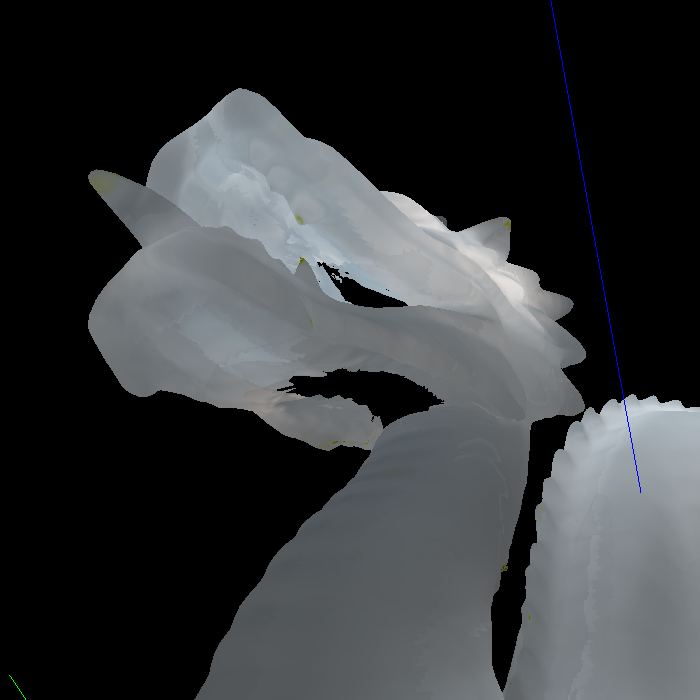
\includegraphics[width=350px]{missing.png}
\caption{Some areas in the rendering are not covered.}
\label{fig:img}
\end{figure}

\clearpage
Secondly, I added some randomness on the GPU, randomizing the rotation of the patter for each pixel. In this way, the line artifacts are removed, at the price of a lot of noise. As we can see, even 1000 samples cannot remove the noise completely (see next picture).


\vspace{0.5cm}
\begin{figure}[!h]
\centering
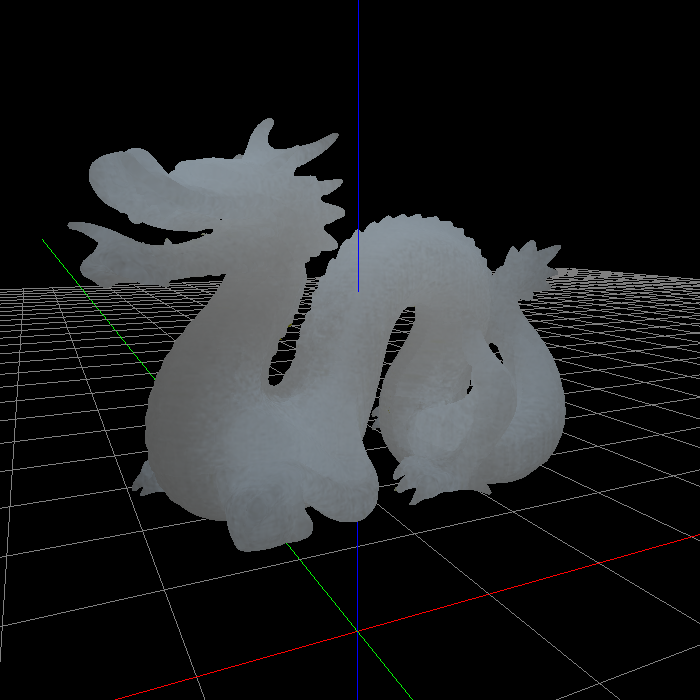
\includegraphics[width=350px]{jensen_1000_onepass.png}
\caption{Randomized rotation of pattern. Jensen's Dipole, 1000 samples.}
\label{fig:img}
\end{figure}

\clearpage
Finally, I added a time evolution of the pattern. A limited number of points is used, but for each frame the points are rotated progressively around. In addition, a small perturbation of the radius is added, in order to avoid artifacts. The schema I have adopted is illustrated in the following picture:


\clearpage
This, at convergence (100 frames, 120 samples per frame), gives me the following results. Each frame during the evolution of the system takes about 50ms with the directional dipole and 40ms with Jensen's dipole.

%\begin{figure}[!ht]
%\centering
%\subfloat[Uniform]{
  %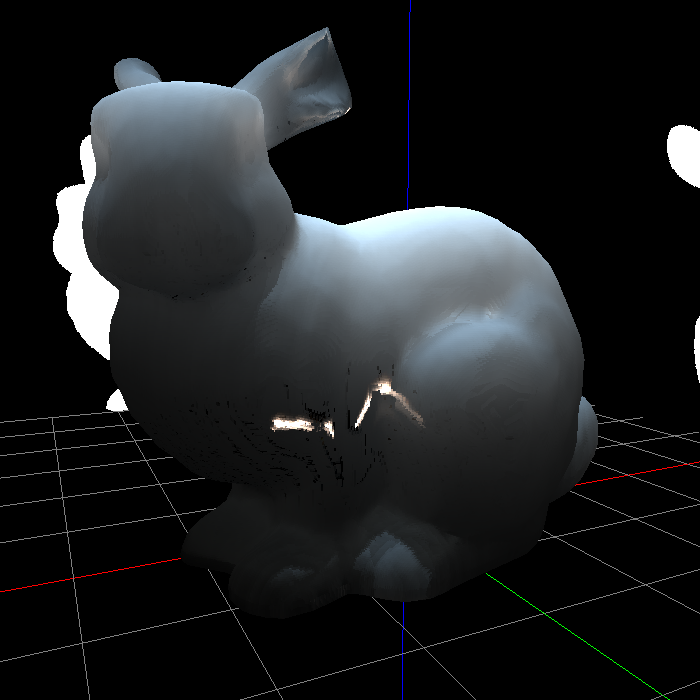
\includegraphics[width=0.5 \linewidth]{bunny_jeppe_uniform.png}
  %\label{fig:ss2}
%} 
%\subfloat[Exponential]{
  %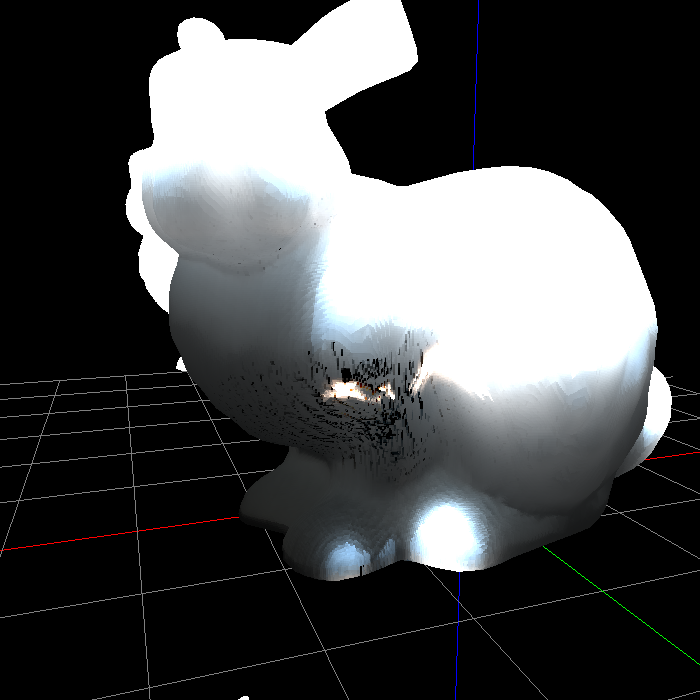
\includegraphics[width=0.5 \linewidth]{bunny_jeppe_exp.png}
  %\label{fig:ss3}
%}
%\\
%\subfloat[Uniform]{
  %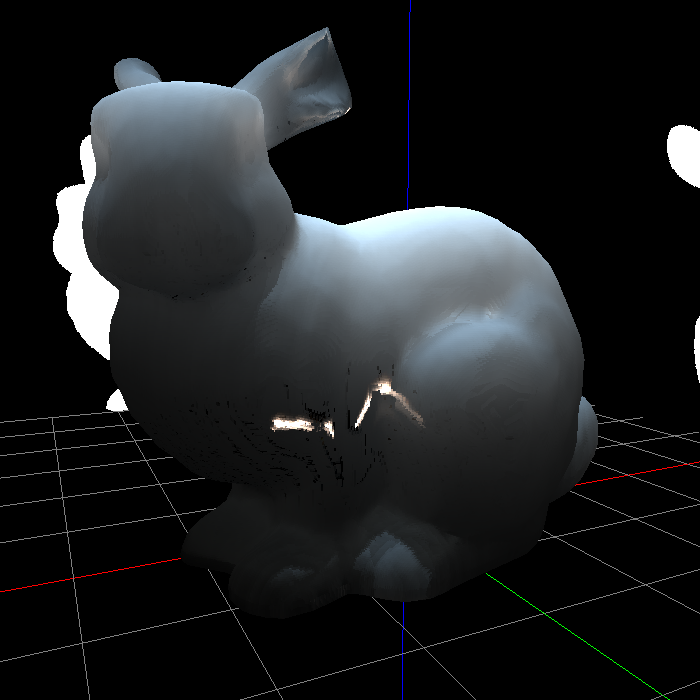
\includegraphics[width=0.5 \linewidth]{bunny_jeppe_uniform.png}
  %\label{fig:ss2}
%} 
%\subfloat[Exponential]{
  %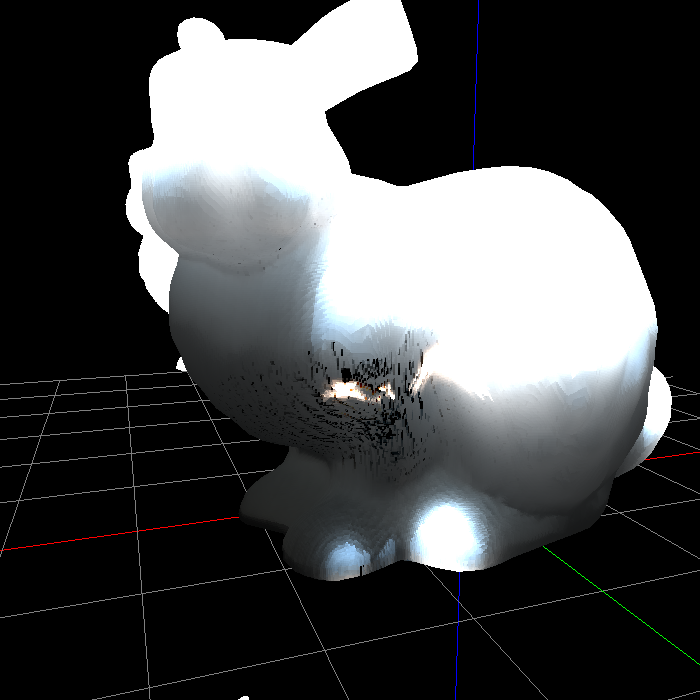
\includegraphics[width=0.5 \linewidth]{bunny_jeppe_exp.png}
  %\label{fig:ss3}
%}
%\caption{This week results.}
%\label{fig:img}
%\end{figure}

\clearpage

\begin{figure}[!h]
\centering
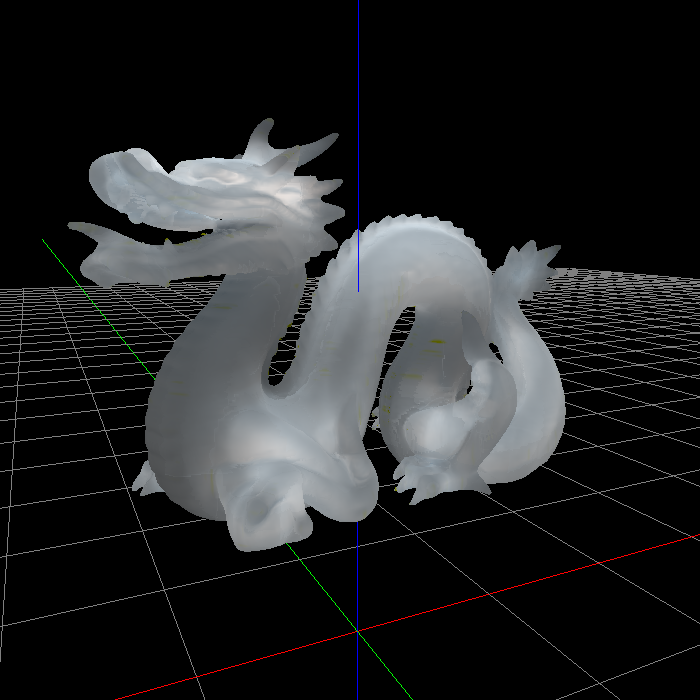
\includegraphics[width=350px]{jeppe_120_100_frames.png}
\caption{Directional dipole.}
\label{fig:img}
\end{figure}

\clearpage
A possible solution for solving the noisiness of the first stages would be to use mipmaps to get a basic filtering of the image. In fact, mipmaps act as a simple box-filter, that eliminates high frequency noise - what we want. I tried to apply it, but the problem is that the black color outside the model starts bleeding inside, ruining the result. I need to implement then my own mipmap generation if I want to use this technique.

\vspace{0.5cm}
\begin{figure}[!h]
\centering
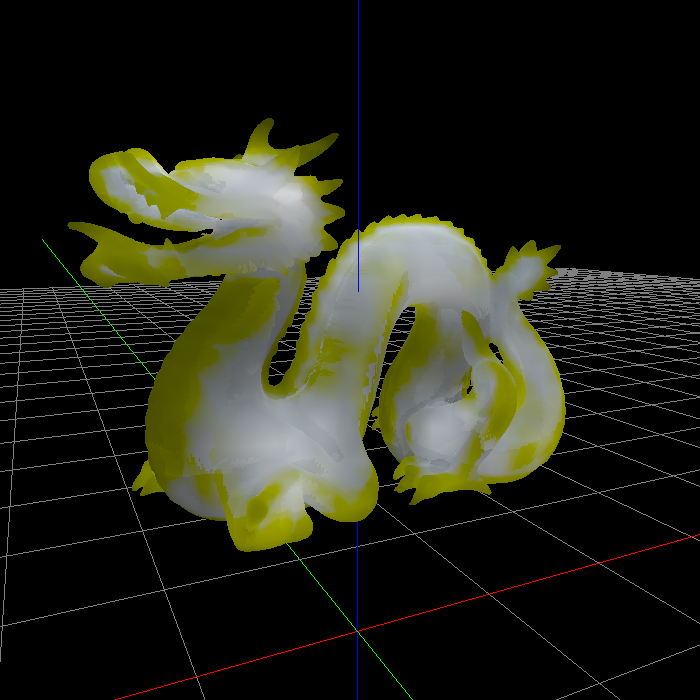
\includegraphics[width=350px]{lod.png}
\caption{Color bleeding happens when we tried to use the low order mipmaps.}
\label{fig:img}
\end{figure}


\clearpage
\section{Future work}
Next steps that I would like to take in the domain of \textit{quality}:

\begin{itemize}
	\item Number of cameras and their placement: where should they be? (Difficulty: Hard)
	\item Using an A-buffer with OpenGL 4.2 capabilities: to test and see, it would eliminate the problem of the cameras. (Difficulty: Medium)
	\item Investigate time and sampling patterns that may help a faster convergence. (Difficulty: ?)
	\item Manual generation of mipmaps, in order to include a border to limit the bleeding effect. (Difficulty: Medium)
	\item Multiple lights and introduction of point lights (Difficulty: Easy)
\end{itemize}

Next steps that I would like to take in the domain of \textit{performance}:

\begin{itemize}
	\item General optimization in shaders (mostly numerical)
	\item Random numbers using texture instead of deterministic GPU generation.
	\item Optimize the rendering to texture array/cubemap to be in only one pass.
\end{itemize}
%
%\textbf{Documents}: Finished Related Work and started Implementation sections.
%
%\textbf{Code}: I investigated more on the possible sampling patterns that are used in the models, as well as reasoning on the formula for efficiently integrating the equations.
%
%At the end I came up with this formula:
%$$
%L(\mathbf{x}_o, \vec{\omega}_o) = \frac{A_{circle}}{k}\sum_{i = 1}^{k}S_i(\mathbf{x}_i,\mathbf{x}_o,\vec{\mathbf{\omega}}_i, \vec{\mathbf{\omega}}_o) \; (n_i\cdot \vec{\mathbf{\omega}}_i) \; F_t(n_i,\vec{\mathbf{\omega}}_i)
%$$
%
%where $A_{circle}$ is the area of the circle in world space. I used the following two sampling patterns, an uniform one and an exponential one. Both are generated using Hammersmith points, the second is modified by converting the points to polar coordinates and then applying the following formula to the radius:
%
%$$
%r^{*} =  \frac{e^{\sigma r} - 1}{e^{\sigma} - 1}; 
%$$
%
%We used $\sigma = 2$ for all tests. We tested different radiuses in texture space with both the exponential and uniform pattern.
%
%\clearpage
%\begin{figure}[!ht]
%\centering
%\subfloat[Uniform]{
  %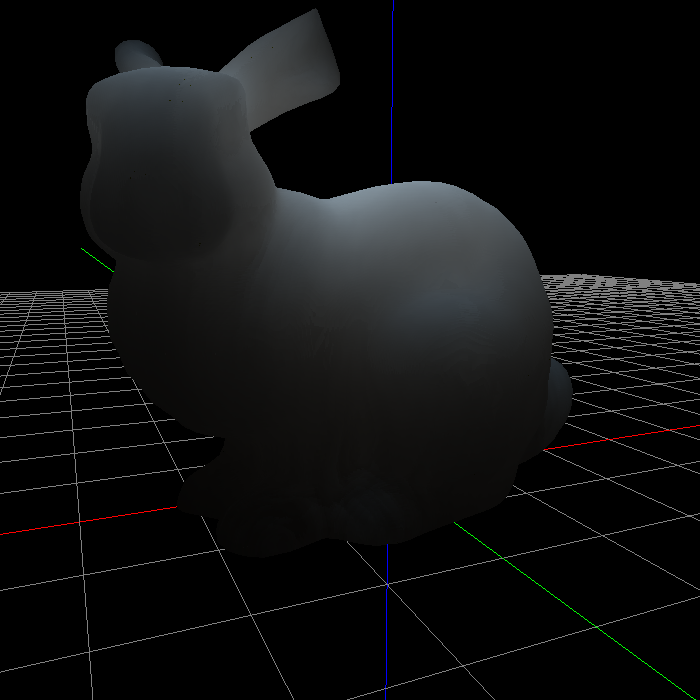
\includegraphics[width=0.33 \linewidth]{radius_03_500_uniform.png}
  %\label{fig:ss2}
%} 
%\subfloat[Exponential]{
  %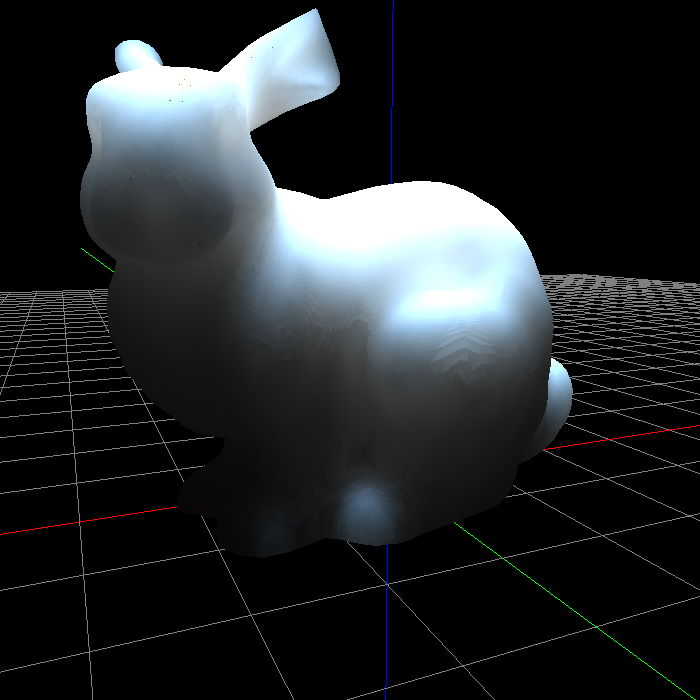
\includegraphics[width=0.33 \linewidth]{radius_03_500.png}
  %\label{fig:ss3}
%}
%\subfloat[Reference]{
  %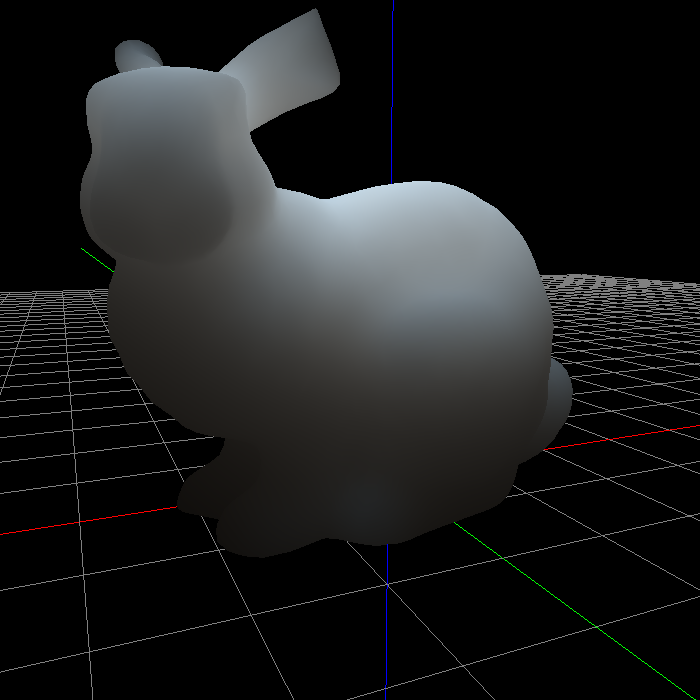
\includegraphics[width=0.33 \linewidth]{reference}
  %\label{fig:ss3}
%} 
 %
%\caption{Difference between sampling patterns vs. reference. Jensen dipole, $r = 0.3$, 300 samples.}
%\label{fig:img}
%\end{figure}
%
%\begin{figure}[!ht]
%\centering
%\subfloat[Uniform]{
  %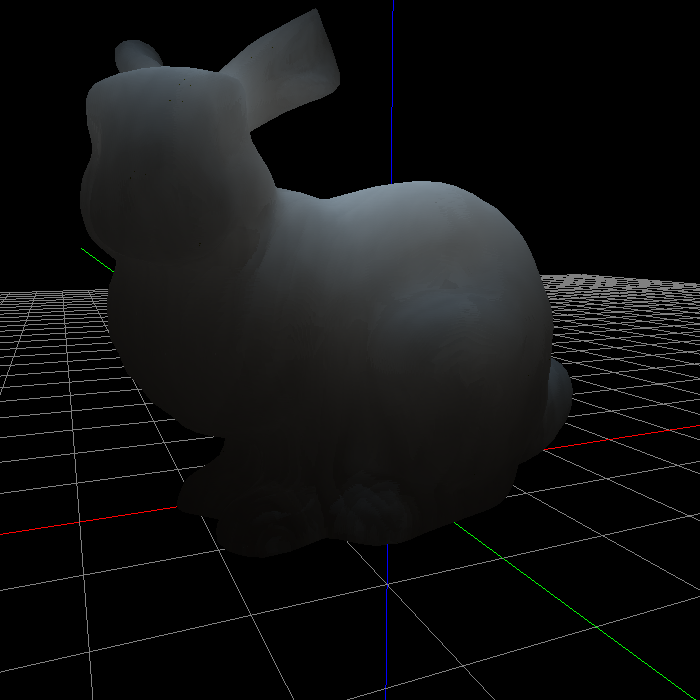
\includegraphics[width=0.33 \linewidth]{radius_05_500_uniform.png}
  %\label{fig:ss2}
%} 
%\subfloat[Exponential]{
  %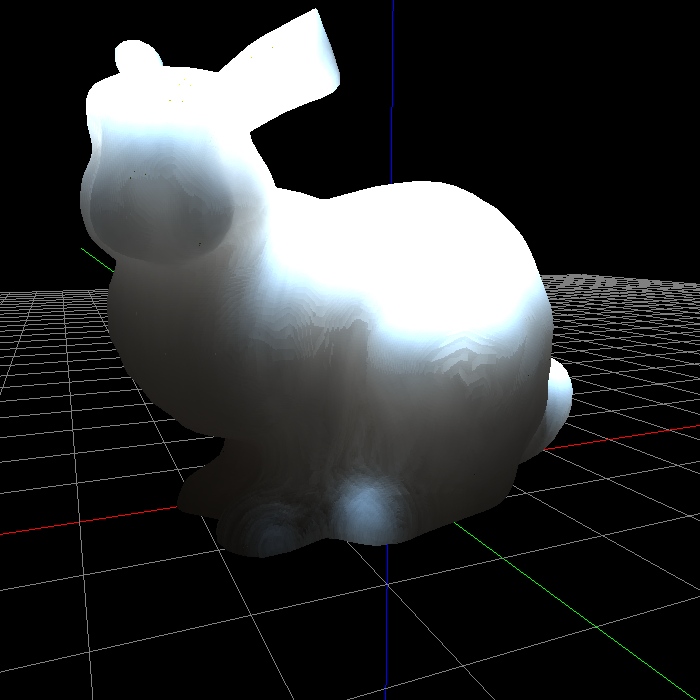
\includegraphics[width=0.33 \linewidth]{radius_05_500.png}
  %\label{fig:ss3}
%}
%\subfloat[Reference]{
  %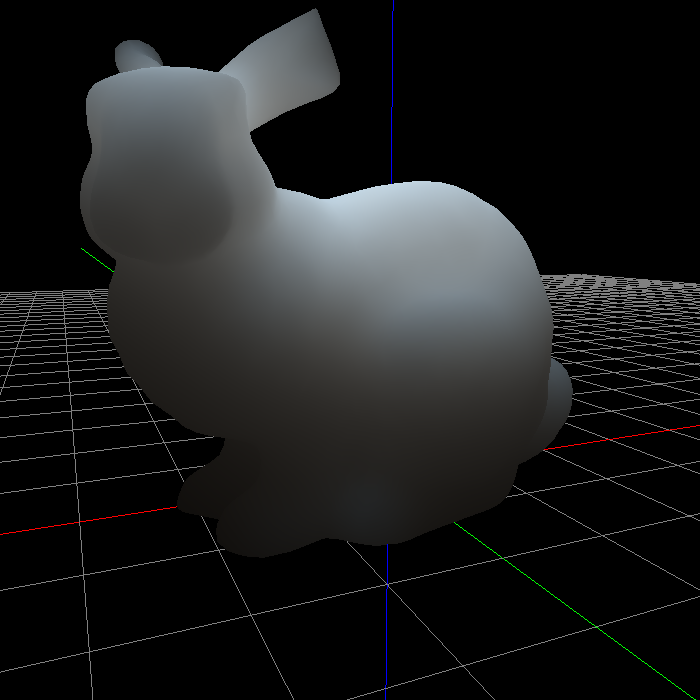
\includegraphics[width=0.33 \linewidth]{reference}
  %\label{fig:ss3}
%} 
 %
%\caption{Difference between sampling patterns vs. reference. Jensen dipole, $r = 0.5$, 300 samples.}
%\label{fig:img}
%\end{figure}
%\clearpage
%
%In the implementation with directional dipole, there are still some artifacts, that need investigation.
%\begin{figure}[!ht]
%\centering
%\subfloat[Uniform]{
  %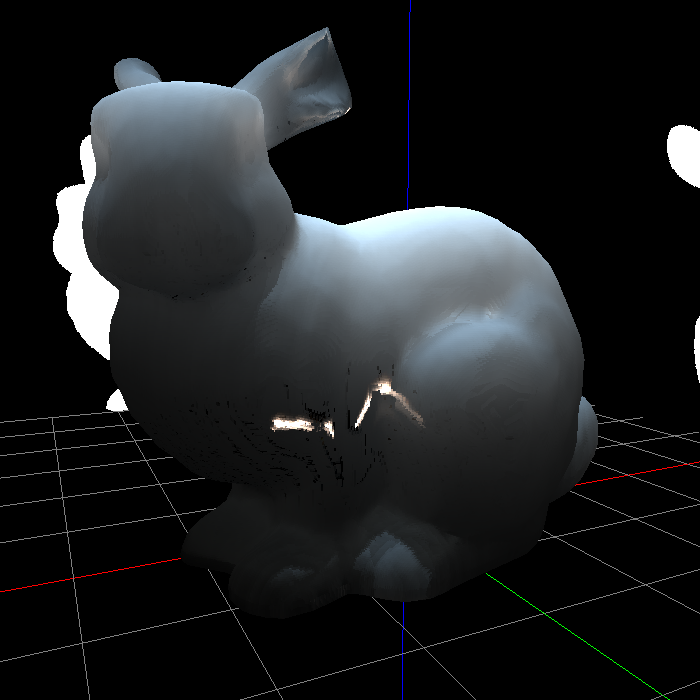
\includegraphics[width=0.5 \linewidth]{bunny_jeppe_uniform.png}
  %\label{fig:ss2}
%} 
%\subfloat[Exponential]{
  %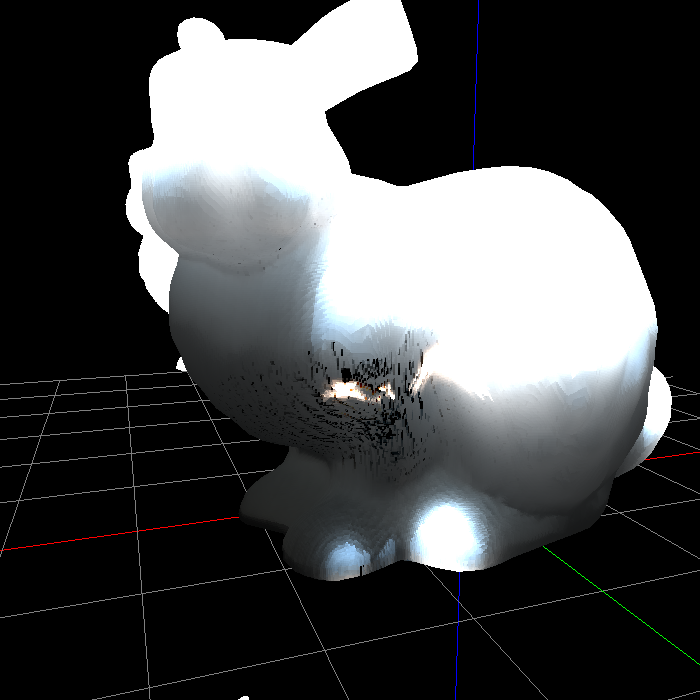
\includegraphics[width=0.5 \linewidth]{bunny_jeppe_exp.png}
  %\label{fig:ss3}
%}
 %
%\caption{Difference between sampling patterns. Directional dipole, $r = 0.5$, 1000 samples.}
%\label{fig:img}
%\end{figure}
%
%


\end{document}
